\subsection{Tick}

Die Simulation behandelt das Verstreichen von Zeit in Zeitschritten, während dem der interne Zustand der Simulation, bzw.~der simulierten Objekte, zu einem zeitlich neuen Zustand aktualisiert wird.
Dieser Zeitschritt, bzw.~Verarbeitungsschritt, wird oft als Tick bezeichnet.\\

Es ist besonders anzumerken, das der Begriff des Ticks sich ausschließlich auf das Voranschreiten der Simulation bezieht und nicht dem Anzeigen einer Szene. Die Äquivalente Bezeichnung im Kontext der Grafik wird als Frame bezeichnet, in welchem eine Szene (ein Grafischer Zustand der Simulation) gerendert wird. Es besteht Verwechslungsgefahr. Von beiden Größen können Raten $r_{tick}, r_{frame}$ angegeben werden (üblicherweise in Tick/Frame pro Realzeitsekunde). Praktisch kann eine Grafikengine durch Inter- oder Extrapolation dynamisch verschiedene, von der Tickrate unabhängige Frameraten erreichen.\\
Wir definieren die Menge der Ticks $\delta:T_r^2; \delta:=\{\delta_1, \delta_2, ...\}$ anhand ihrer Start- und Endzeitpunkte in Echtzeit $\delta_i := (\delta_{i0}, \delta_{i1})$ und erweitert die zu einem Tick gehörenden Zeitpunkte als $\delta_{id}; d \in [0,1]$. Die Inklusivität/Exklusivität muss in bestimmten Berechnungskontexten manchmal angepasst werden um bei sukzessiven Ticks doppelte Behandlungen von Ereignissen zu vermeiden. Diese Einschätzung sei für jeden Kontext individuell zu vollziehen.\\
Es gilt außerdem die Kontinuität der Zeit auch bei Ticks $\delta_{j1} = \delta_{(j+1)0}$, d.h. ein Tick beginnt am Endzeitpunkt des Vorherigen.\\
Durch die Abbildung $\mathcal{T}$ erhält der Tick eine Entsprechung in Simulationszeit.\\
Ist im aktuellen Kontext nur ein Tick $\delta_i$ von Belang, wird auch die Terminologie $t_d =\mathcal{T}(\delta_{id})$, also $t_0$ für den Tickbeginn und $t_1$ für dessen Ende in Simulationszeit, verwendet.\\
Man kann weiter die Sequenz $\Upsilon_{\delta i} = \langle t_0, ...,  t_1\rangle$ als die zusammenhängende Partition der Simulationszeitsequenz $T_s$ denotieren, welche die geordneten Zeitpunkte eines Ticks in Simulationszeit enthält.\\
Die in Abschnitt~\ref{sec:time} beschriebenen möglichen Umschaltzeiten zur Änderung der Zeitflussrate in der Simulation werden auf die Grenzen von Ticks gelegt.\\
Die Größe der Zeitdifferenz $t_1 - t_0$ unterliegt meist Einschränkungen. Bestimmte Simulationsalgorithmen wie z.B. die Methode der kleinen Schritte erfordern für eine bestimmte Genauigkeit eine maximale Schrittgröße. Die verfügbare Rechenleistung hingegen beschränkt die Tickrate nach oben. Reicht die Berechnungszeit während eine Ticks nicht um den Status der Simulation von $t_0$ auf $t_1$ zu aktualisieren, läuft die Simulation langsamer als die reale Zeit. Die Echtzeitanforderung ist dann verletzt. Oft wird die Tickrate als Konstante festgelegt, in diesem Projekt ist jedoch nur eine Mindestrate festgelegt.\\
Das Konzept eines Ticks und dessen Mindestrate war schon vor dem Projekt in der Codebasis enthalten, die Implementierung erfuhr jedoch einige Anpassungen.

\subsection{Hitbox}
\label{sec:hitbox}
Hitboxen sind Approximationen für Modelle in einer Simulation. Sie ersetzen das konkrete Modell dabei für Kollisionen gegenüber der Kollisionserkennung komplett.\\
Der Term Hitbox suggeriert die verwendung einer Box/eines Quaders zur Approximation. Das ist historisch bedingt. Der Term ist allerdings auch für andere Approximationsformen etabliert.\\
Die Diskrepanz zwischen Hitbox und Model wirkt sich negativ auf den physikalischen Realismus aus. Trotzdem wird von Entwicklern so viel wie kontextuell vertretbar approximiert, um Rechenzeit zu sparen und Echtzeitanforderungen zu genügen.

\begin{figure*}
	\begin{subfigure}[t]{0.45\textwidth}
		\centering
		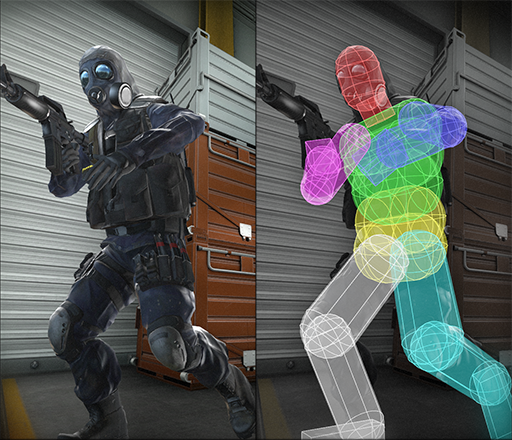
\includegraphics[width=1\textwidth]{./res/csgo_hitbox.png}
		\caption{Hitbox des Spieler-Modells aus dem Videospiel Counter Strike: Global Offensive; sichtbares Modell(links), mit eingeblendeter Hitbox (rechts)}
%%TODO source for pic
		\label{fig:chitbox}
	\end{subfigure}
~
	\begin{subfigure}[t]{0.2\textwidth}
		\centering
		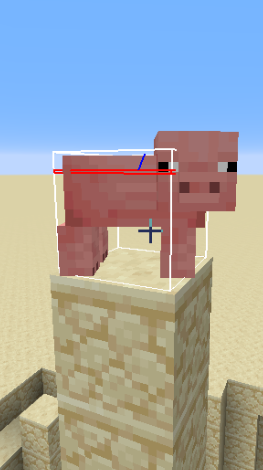
\includegraphics[width=1\textwidth]{./res/pig_hitbox.png}
		\caption{Hitbox eines NPC-Modells (Schwein) aus dem Videospiel Minecraft; Hitbox in weiß}
		\label{fig:mphitbox}
	\end{subfigure}
~
	\begin{subfigure}[t]{0.2\textwidth}
		\centering
		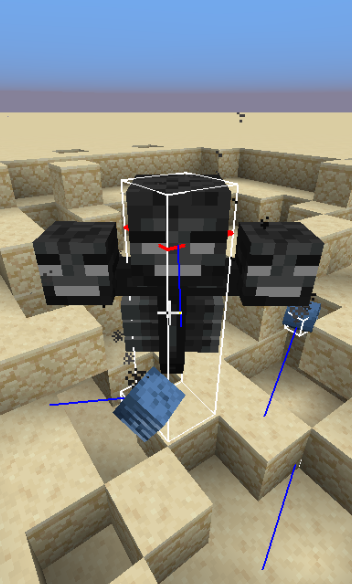
\includegraphics[width=1\textwidth]{./res/wither_hitbox.png}
		\caption{Hitbox eines NPC-Modells (Wither) aus dem Videospiel Minecraft; Hitbox in weiß}
		\label{fig:mwhitbox}
	\end{subfigure}

	\caption{Güten von Hitboxen}
	\label{fig:hitbox}
\end{figure*}

Die Abbildungen~\ref{fig:hitbox} zeigen Hitboxen in 2 verschiedenen Spielen.\\
\ref{fig:chitbox} zeigt das Spielermodell aus dem Spiel Counter-Strike: Global Offensive (CSGO). Links ist dabei das sichtbare Modell zu sehen, während rechts die Hitboxen eingeblendet sind. Die Hitboxen, welche hier nichmal mehr Boxen sind, sondern Ellipsoiden, decken das sichtbare Modell relativ genau ab. Ebenfalls zu erkennen ist die Partition in einzelne Hitboxen, zu sehen an den verschiedenen Farben der Hitboxen im rechten Bild.\\
Einzelne Details des Spielermodells, wie Riemen und Taschen an der Ausrüsung, sind nicht essentiell und werden daher auch physikalisch nicht abgebildet.\\
\ref{fig:mphitbox} und \ref{fig:mwhitbox} zeigen Hitboxen aus dem Spiel Minecraft bei zwei NPCs (Non-Player-Character (zu Deutsch: Nicht-Spieler-Charakter)). Es ist dort klar zu erkennen, dass die Hitboxen nicht sehr genau mit dem sichtbaren Modell übereinstimmen. Mehr noch: Die Minecraft-Hitboxen sind Koordinatenachsenparallel, d.h. Kanten verlaufen immer entlang der Koordinatenachsen der Raumrepräsentation.\\
Es wird versucht die Unterschiede zu rechtfertigen:\\
CSGO ist ein Shooter. Schnelle Reaktion und genaues Zielen sind ein hauptbestandteil des Produkts. Zudem ist CSGO ein hochkompetitiver E-Sport, der professionell gespielt wird. Es geht dabei um Preisgelder im siebenstelligen Bereich \cite{csgoprice}. Akkurate und, aus der perspektive des Spielers deterministische Hitboxen sind daher essenziell für das Produkt.\\
Die Partition der Hitboxen in CSGO ergibt sich direkt aus einer Anforderung der Anwendung, Schusstreffer auf verschiedene Teile des Spielermodells unterschiedlich zu bewerten. Beispielsweise verursacht der Treffer am Kopf am meisten Schaden. CSGO modelliert die unterschiedlichen Treffbaren teile des Modells also über mehrere Hitboxen.\\
Minecraft ist ein Sandbox Aufbauspiel. Ziel des Spiels ist der Bau von beliebigen Gebäuden, Tunneln, die Kreation von Maschinen oder das Erkunden von Gebieten.\\
In Minecraft steckt auch eine erhebliche Summe Geld. Am 15. September 2014 kaufte Microsoft die Entwicklerfirma und die rechte am Spiel für ca. 2,5 Milliarden Dollar \cite{buyminecraft}.\\
Das Kampfsystem in Minecraft forciert keine schnellen und genauen Treffer auf Gegner. Die gesamte Spielwelt ist aus sichtbaren Achsenparallel aufgestellten Würfeln gegeben, sind also Deckungsgleich mit entsprechenden achsenparallelen Hitboxen. Minecraft macht es sich einfach, da keine konkreten Anforderungen hinsichtlich Genauigkeit bestehen. Tatsächlich wird eine künstlich kleinere Hitbox manchmal sogar eingesetzt um einen Treffer zu erschweren (vgl. Abbildung \ref{fig::mwhitbox}).\\


\subsection{Double Buffering}
\label{sec:doublebuffer}
Beim grafischen Rendern einer Szene werden übicher weise mehrere (hier 2) Buffer angelegt, in welche die Szene gezeichnet wird.\\
Dabei ist ein Buffer der Renderbuffer, zu dem aktiv gezeichnet wird,\\
der andere ist der Displaybuffer, welcher zur Anzeige aktivgeschaltet ist und dann in einem Fenster angezeigt werden kann.\\
Nach einem volzogenen Rendering-Vorgang werden die Rollen der Buffer vertauscht und der nächste Rendering-Schritt durchgeführt. Dieser Zyklus wird Grafiktick genannt (siehe \ref{sec:tick})\\
Dieses Verfahren wird verwendet um Race-Conditions auf den Buffer zu vermeiden, was sichtabre flickernde Fragmente im Ausgabebild erzeugen kann.
